\begin{figure*}
  \begin{minipage}{0.6\textwidth}
    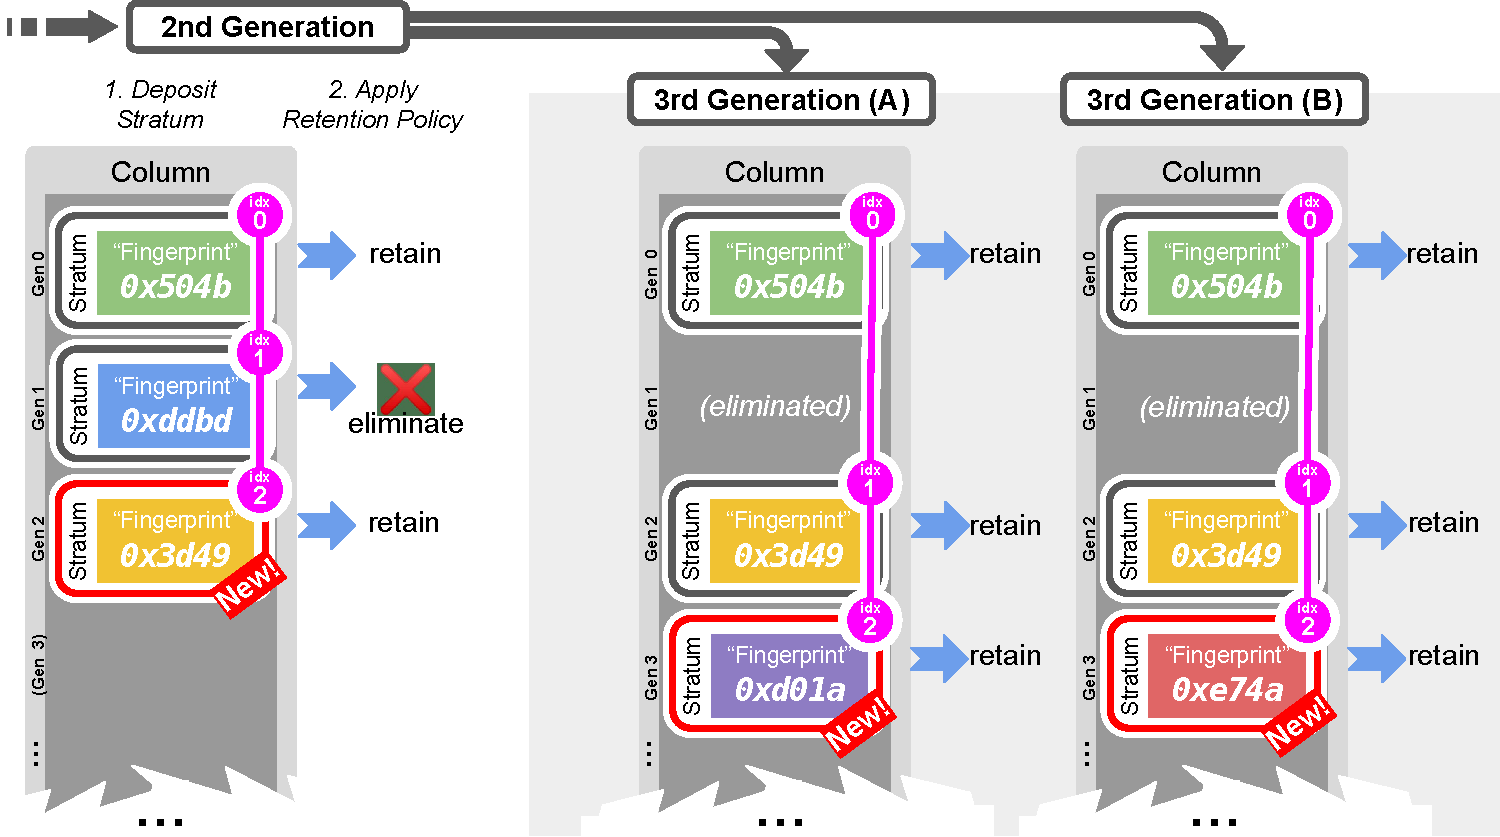
\includegraphics[width=\textwidth]{img/deposit-process}
  \end{minipage}%
  \begin{minipage}{0.4\textwidth}
    \caption{
    Cartoon illustration of stratum deposit process.
    This process marks the elapse of a generation when a hereditary stratigraphic column is inherited by an offspring.
    First, a new stratum is appended to the end of the column with a randomly-generated ``fingerprint.''
    This ``fingerprint'' distinguishes strata that were generated along disparate lines of descent (e.g., \texttt{0xd01a} for 3rd Generation A and \texttt{0xe74a} for 3rd generation B).
    Then, the column's configured stratum retention policy is applied to ``prune'' the column by eliminating strata from specific generations.
    Although this cartoon depicts an empty space for eliminated strata, the underlying data structure behind a column (i.e., the pink overlay) can condense to reduce space complexity.
    }\label{fig:deposit-process}
  \end{minipage}
\end{figure*}
